
%\documentclass[a4paper,man,apacite,floatsintext,donotrepeattitle]{apa6}
\documentclass[a4paper,man,apacite,donotrepeattitle]{apa6}

\usepackage[ngerman, english]{babel}
\usepackage[utf8]{inputenc}
\usepackage{setspace}
%\usepackage[table,xcdraw]{xcolor}
\usepackage{pdflscape} %turn tables sideways
\usepackage{rotating}
\usepackage{varwidth} %sideways captions
\usepackage{geometry}
\usepackage{amsmath}
\usepackage{footnote}
\usepackage{bm} %bold font in equations
\usepackage[flushleft]{threeparttable} %notes under tables
%tikz
\usepackage{tikz}
\usetikzlibrary{calc, positioning, shapes, arrows}
%Times New Roman
%\usepackage{fontspec}
%\setmainfont{Times New Roman}
\usepackage{xcolor}

\newcommand{\E}{\mathrm{E}}
\newcommand{\Var}{\mathrm{Var}}
\newcommand{\Cov}{\mathrm{Cov}}


\raggedbottom % Formatting

%Title Page
\title{How Response Times Should Inform Test Assembly: A Note on the Speed Sensitivity Parameter in Response Time Modeling
\vspace{3cm}}
\shorttitle{Speed Sensitivity in High Stakes Testing}
\author{\color{white}.}
\affiliation{\color{white}.}



\begin{document}

\appendix

\section{Derivation of the (Model Implied) Correlation of Item Response Times}
In the following, $\lambda_{k}$ and $\phi_{k}$ are the time intensity parameter and the speed sensitivity parameter of item $k$, respectively, $\sigma^2_{\epsilon_{k}}$ is the residual variance parameter of item $k$ and $\zeta_i$ is the speed parameter of person $i$. We assume that over persons, speed is normally distributed $\zeta \sim \mathcal{N}(0, \sigma^2_{\zeta})$. Further, if $X$ is a log normally distributed variable with parameters $\mu$ and $\sigma$, then $X = \exp(Y)$ where $Y \sim \mathcal{N}(\mu, \sigma^2)$, which is the same as $ln(X) \sim \mathcal{N}(\mu, \sigma^2)$. Then, from \citeA{johnson.1994}, the expectation of $X$ is:
\begin{equation}
\label{ElogNorm}
\begin{split}
\E(X) & = \E[\exp (Y)] \\
      & = \exp \left(\mu + \frac{\sigma^2}{2} \right). \\
\end{split}
\end{equation}

In addition, the expectation of $X^2$ is: 
\begin{equation}
\label{E2logNorm}
\begin{split}
\E(X^2) & = \E[(\exp (Y))^2] \\
        & = \E[\exp (2Y)] \\
        & = \E[\exp (Y^*)] \\        
        & = \exp \left(2 \mu + 2 \sigma^2 \right), \\
\end{split}
\end{equation}
where $Y^* = 2Y$ and hence $Y^* \sim \mathcal{N}(2\mu, 4\sigma^2)$.

Based on the 3PLN lognormal measurement model for response times $RT_{ik}$, the expectation of the response time variable $\E(RT_k)$ of an item $k$ can be written as
\begin{equation}
\label{meanRT}
\begin{split}
\E(RT_k) & = \E \left[ \E(RT_{ik} | \zeta_i)  \right] \\
         & = \E \left[ \exp \left( \lambda_{k} - \phi_{k} \zeta_i + \frac{\sigma^2_{\epsilon_{k}}}{2} \right) \right]  \\
         & = \E \left[ \exp( Z ) \right] \\
         & = \exp \left( \lambda_{k} + \frac{\sigma^2_{\epsilon_{k}}}{2} + \frac{\phi^2_{k} \sigma^2_{\zeta}}{2} \right),
\end{split}
\end{equation}
where $Z$ is a normally distributed: $ Z \sim \mathcal{N} (\lambda_{k} + \frac{\sigma^2_{\epsilon_{k}}}{2}, \phi^2_{k} \sigma^2_{\zeta})$.

Using similar steps in the derivation, the expectation of the squared response time variable $\E(RT^2_k)$ can be written as
\begin{equation}
\label{meanRT2}
\begin{split}
\E[RT^2_k] & = \E \left[ \E(RT^2_{ik} | \zeta_i)  \right] \\
           & = \E \left[ \exp \left( 2 \lambda_{k} - 2 \phi_{k} \zeta_i + 2 \sigma^2_{\epsilon_{k}} \right) \right]  \\
           & = \exp \left( 2 \lambda_{k} + 2 \sigma^2_{\epsilon_{k}} + 2 \phi^2_{k} \sigma^2_{\zeta} \right) \\
\end{split}
\end{equation}

Therefore the variance of the response time variable of item $k$, $\Var(RT_k)$, can be denoted as
%- \exp \left( 2 \lambda_{k} + \sigma^2_{\epsilon_{k}} + \phi^2_{k} \sigma^2_{\zeta} \right)
\begin{equation}
\label{VarRT}
\begin{split}
\Var(RT_k) & = \E(RT^2_k) - \E(RT_k)^2 \\ 
           & = \exp \left( 2 \lambda_{k} + 2 \sigma^2_{\epsilon_{k}} + 2 \phi^2_{k} \sigma^2_{\zeta} \right) - \exp \left( 2 \lambda_{k} + \sigma^2_{\epsilon_{k}} + \phi^2_{k} \sigma^2_{\zeta} \right) \\
           & = \exp \left( 2 \lambda_{k} \right) \exp \left( \sigma^2_{\epsilon_{k}} + \phi^2_{k} \right) \exp \left( \sigma^2_{\epsilon_{k}} + \phi^2_{k} \right) - \exp \left( 2 \lambda_{k} \right) \exp \left( \sigma^2_{\epsilon_{k}} + \phi^2_{k} \right) \\
          & = \exp \left( 2 \lambda_{k} + \sigma^2_{\epsilon_{k}} + \phi^2_{k} \sigma^2_{\zeta} \right) \left( \exp(\sigma^2_{\epsilon_{k}} + \phi^2_{k} \sigma^2_{\zeta}) - 1 \right) \\
\end{split}
\end{equation}

For the expectation of the distribution of the product of the response times of items $k$ and $l$, $\E(RT_k RT_l)$, this gives
\begin{equation}
\label{meanRTRT}
\begin{split}
\E(RT_k RT_l) & =   \E \left[ \exp \left( N( \lambda_{k} +  \lambda_{l} - (\phi_{k} + \phi_{l}) \zeta, \sigma^2_{\epsilon_{k}} + \sigma^2_{\epsilon_{l}} )\right) \right] \\
               & = \exp \left( \lambda_{k} + \lambda_{l} +  \frac{\sigma^2_{\epsilon_{k}} + \sigma^2_{\epsilon_{l}}}{2} + \frac{(\phi_{k} + \phi_{l})^2 \sigma^2_{\zeta}}{2} \right) \\  
\end{split}
\end{equation}

Therefore the covariance of the response time variables of two items $k$ and $l$, $\Cov(RT_k, RT_l)$ and the respective product of the variances of these two items can be denoted as
\begin{equation}
\begin{alignedat}{1}
\label{CovRT}
\Cov(RT_k, RT_l) = \E(RT_k RT_l) & - \E(RT_k) \E(RT_k) \\ 
                 = \exp \left( \lambda_{k} + \lambda_{l} + \frac{\sigma^2_{\epsilon_{k}} + \sigma^2_{\epsilon_{l}}}{2} + \frac{(\phi_{k} + \phi_{l})^2 \sigma^2_{\zeta}}{2} \right) & - \exp \left( \lambda_{k} + \lambda_{l} + \frac{\sigma^2_{\epsilon_{k}} + \sigma^2_{\epsilon_{l}}}{2}  + \frac{(\phi_{k}^2 + \phi_{l}^2) \sigma^2_{\zeta}}{2} \right) \\ 
                 =  \exp \left( \lambda_{k} + \lambda_{l} + \frac{\sigma^2_{\epsilon_{k}} + \sigma^2_{\epsilon_{l}}}{2}  + \frac{(\phi_{k}^2 + \phi_{l}^2) \sigma^2_{\zeta}}{2} \right) & \left[ \exp \left( \phi_{k}\phi_{l} \sigma^2_{\zeta} \right) -1 \right]
\end{alignedat}
\end{equation}

\begin{equation}
\begin{alignedat}{2}
\label{VarVar}
\Var(RT_k) \Var(RT_l) \\ & = &&\exp \left( 2 \lambda_{k} + \sigma^2_{\epsilon_{k}} + \phi^2_{k} \sigma^2_{\zeta} \right) \left( \exp(\sigma^2_{\epsilon_{k}} + \phi^2_{k} \sigma^2_{\zeta}) - 1 \right) \\ &\textcolor{white}{x} &&\exp \left( 2 \lambda_{l} + \sigma^2_{\epsilon_{l}} + \phi^2_{l} \sigma^2_{\zeta} \right) \left( \exp(\sigma^2_{\epsilon_{l}} + \phi^2_{l} \sigma^2_{\zeta}) - 1 \right) \\
& = &&\exp \left( 2 \lambda_{k} + \sigma^2_{\epsilon_{k}} + \phi^2_{k} \sigma^2_{\zeta} \right) \exp \left( 2 \lambda_{l} + \sigma^2_{\epsilon_{l}} + \phi^2_{l} \sigma^2_{\zeta} \right) \\ &\textcolor{white}{x} && \left( \exp(\sigma^2_{\epsilon_{k}} + \phi^2_{k} \sigma^2_{\zeta}) - 1 \right)  \left( \exp(\sigma^2_{\epsilon_{l}} + \phi^2_{l} \sigma^2_{\zeta}) - 1 \right) \\
 & = &&\exp \left( 2 \lambda_{k} + 2 \lambda_{l} + \sigma^2_{\epsilon_{k}} +  \sigma^2_{\epsilon_{l}} + \phi^2_{k} \sigma^2_{\zeta} + \phi^2_{l} \sigma^2_{\zeta} \right) \\ &\textcolor{white}{x} &&  \left( \exp(\sigma^2_{\epsilon_{k}} + \phi^2_{k} \sigma^2_{\zeta}) - 1 \right)  \left( \exp(\sigma^2_{\epsilon_{l}} + \phi^2_{l} \sigma^2_{\zeta}) - 1 \right) 
\end{alignedat}
\end{equation}

This gives
\begin{equation}
\begin{split}
\rho_{RT_k, RT_l} & = \frac{\Cov(RT_k, RT_l)}{\sqrt{\Var(RT_k) \Var(RT_l)}} \\
                  & = \frac{\left[ \exp \left( \phi_{k}\phi_{l} \sigma^2_{\zeta} \right) -1 \right]}{\sqrt{\left( \exp(\sigma^2_{\epsilon_{k}} + \phi^2_{k} \sigma^2_{\zeta}) - 1 \right)  \left( \exp(\sigma^2_{\epsilon_{l}} + \phi^2_{l} \sigma^2_{\zeta}) - 1 \right)}}
\end{split}
\end{equation}

This is the model implied correlation of the two response time distributions of items $k$ and $i$ under the 3PLN model. Under the 2PLN model $phi_k = phi_l = 1$, therefore the respective correlation is
\begin{equation}
\frac{\left[ \exp \left( \sigma^2_{\zeta} \right) -1 \right]}{\sqrt{\left( \exp(\sigma^2_{\epsilon_{k}} + \sigma^2_{\zeta}) - 1 \right)  \left( \exp(\sigma^2_{\epsilon_{l}} +  \sigma^2_{\zeta}) - 1 \right)}}
\end{equation}


\section{Item Log Response TIme Distributions}
\begin{figure}
	\begin{center}
	 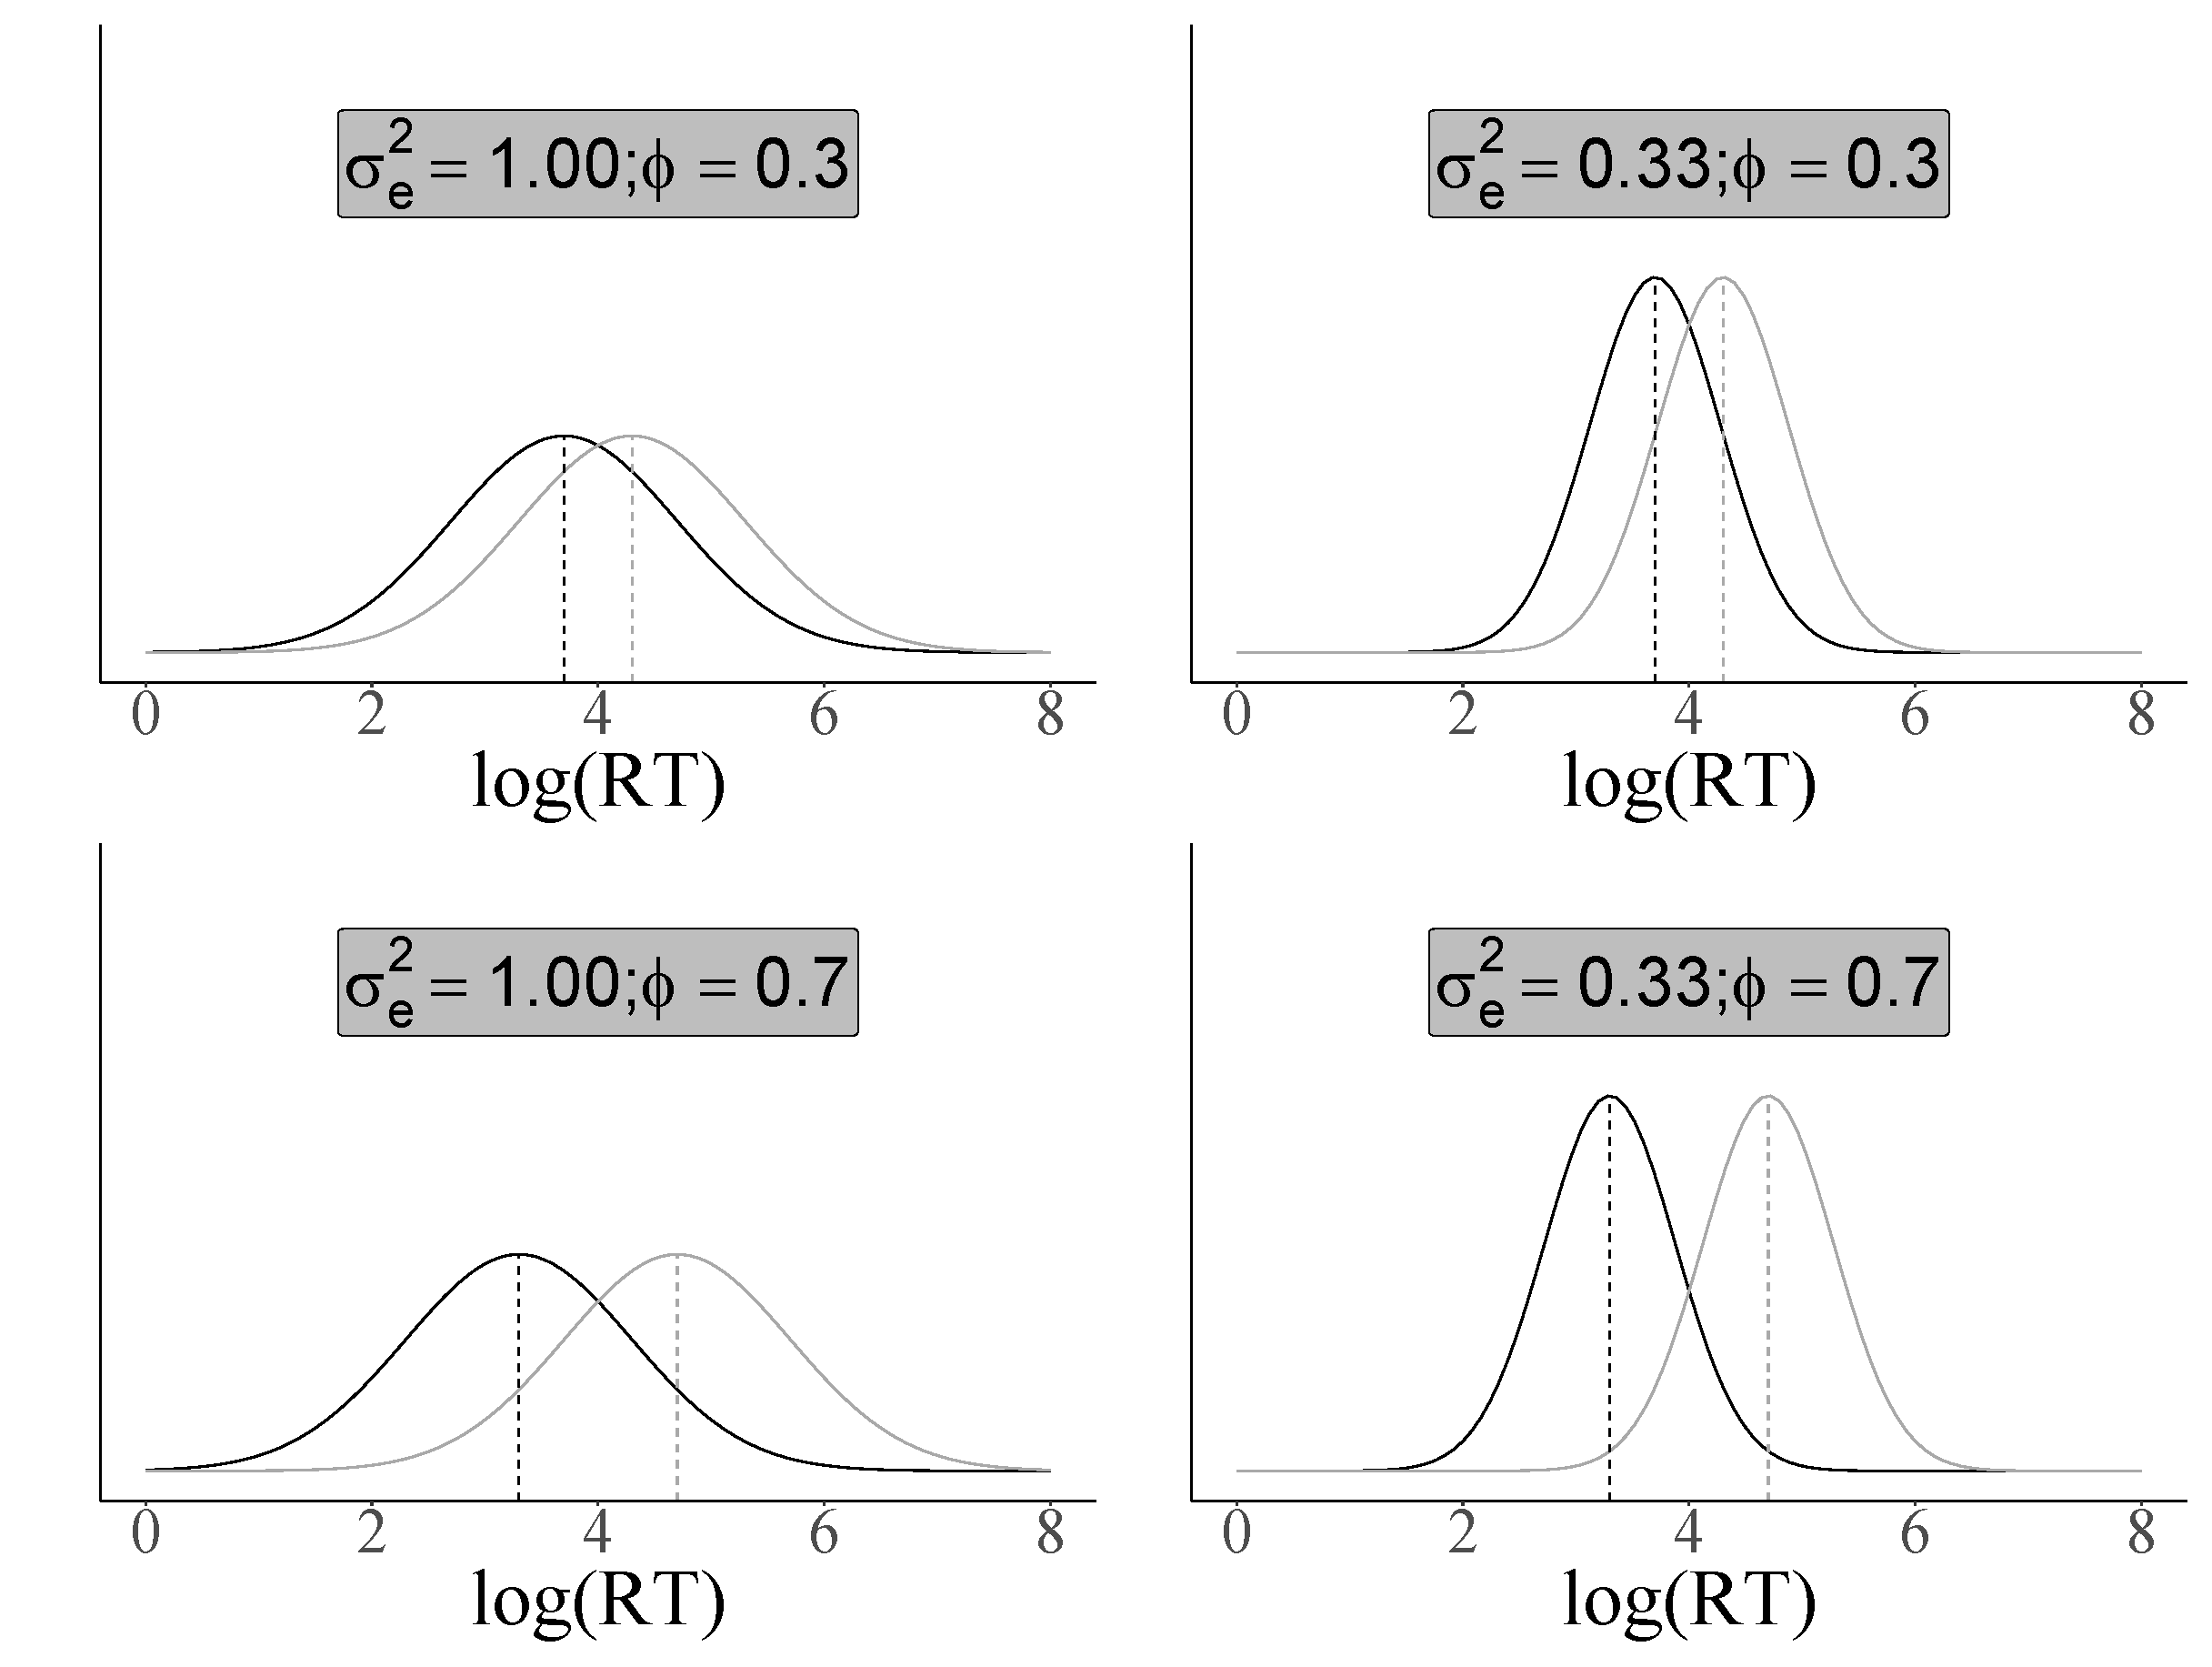
\includegraphics[height = 0.40\textheight]{discrimination_comp_logRT.eps}
	\end{center}		
	 \caption{Expected log response time distributions of a fast person with $\zeta_1 = 1$ (black line) and a slow person with $\zeta_2 = -1$ (grey line) on four different items, all with $\lambda_k = 4$. Dotted lines indicate the medians of the corresponding distributions.} 
	 \label{fig:discr_diff}
\end{figure}

\section{Response Time Characteristic Curve}
\begin{figure}
	\begin{center}
	 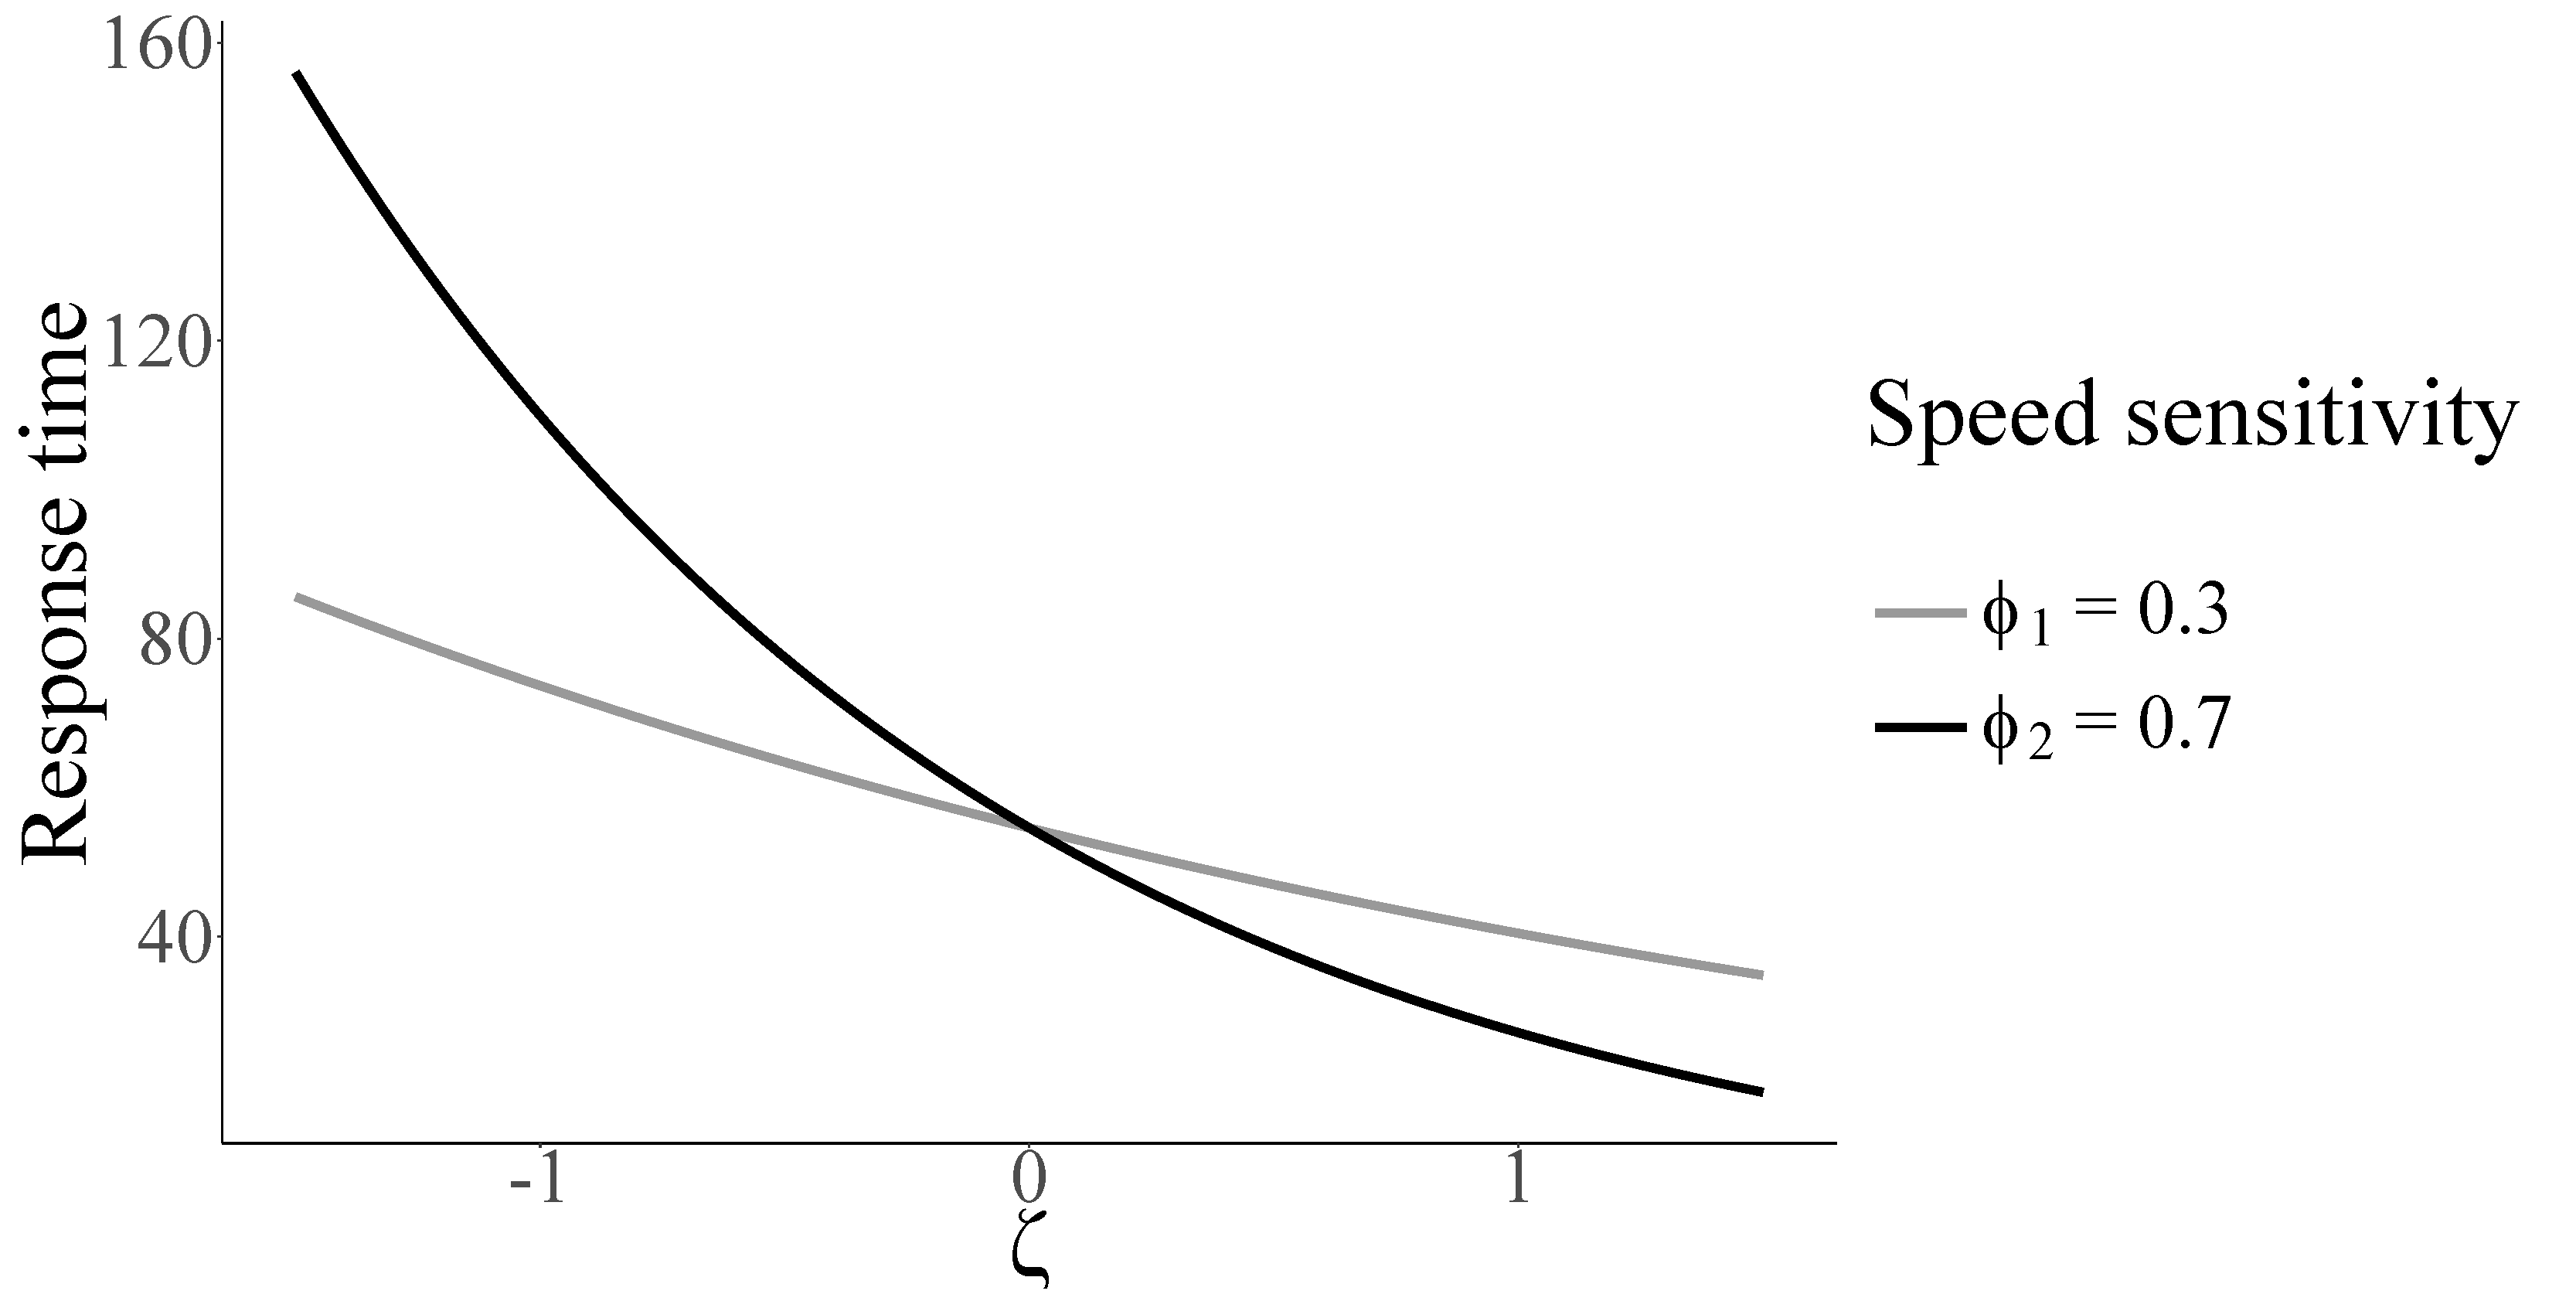
\includegraphics[height = 0.25\textheight]{phi_theoret.eps}
	\end{center}		
	 \caption{Response Time Characteristic Curve of two items with identical time intensity ($\lambda_{k} = 4$) and differing item speed sensitivity parameters $\phi_{k}$.}
	 \label{fig:phi_theoret}
\end{figure}

\section{Priors for Empirical Data Analysis}
The identity matrix is notated as $I_n$ with the size of $n$. $\sigma_{\theta_i, \zeta_i}$ is truncated to stay in range of $-\sqrt{\sigma^2_{\theta}\sigma^2_{\zeta}} $ and $\sqrt{\sigma^2_{\theta}\sigma^2_{\zeta}}$ (with $\sigma^2_{\theta} = 1$ for model identification) to keep the person parameter covariance matrix positive definite.  Priors for the HRT with a 2PL model for ability and a 2PLN model for speed:
\begin{equation}
\begin{gathered}
\Sigma_P \sim InverseWishart(I_3, 4) \\
\sigma_{\theta_i, \zeta_i} \sim N(0, 10000) \text{ truncated at } [-\sigma_{\zeta},\sigma_{\zeta}] \\
\frac{1}{\sigma^2_{\zeta}} \sim \Gamma(0.01, 0.01)  \\
\frac{1}{\sigma^2_{\sigma_{\epsilon}}}  \sim \Gamma(0.01, 0.001) \\
\mu_{\sigma_{\epsilon}} \sim N(0, 1000000) \\
\mu_{b} \sim N(0, 1000000) \\
\mu_{a} \sim N(1, 1000000) \\
\mu_{\lambda} \sim N(1, 1000000)
\end{gathered}
\end{equation}


Priors for the HRT with a 2PL model for ability and a 3PLN model for speed:
\begin{equation}
\begin{gathered}
\Sigma_P \sim InverseWishart(I_4, 5) \\
\sigma_{\theta_i, \zeta_i} \sim N(0, 10000) \\
\frac{1}{\sigma^2_{\sigma_{\epsilon}}} \sim \Gamma(0.01, 0.001) \\
\mu_{\sigma_{\epsilon}} \sim N(0, 1000000) \\
\mu_{b} \sim N(0, 1000000) \\
\mu_{a} \sim N(1, 1000000) \\
\mu_{\lambda} \sim N(1, 1000000) \\
\mu_{\phi} \sim N(1, 1000000) \\
\end{gathered}
\end{equation}

\section{Empirical Model Fit}
% latex table generated in R 3.6.2 by xtable 1.8-4 package
% Fri Jan 31 15:57:54 2020
\begin{table}
\centering
\caption{DIC for the HRT with the 2PLN and the 3PLN and the corresponding difference for all
                    Math booklets.} 
\begin{tabular}{llll}
  \hline
Booklet & $DIC(3PLN)$ & $DIC(2PLN)$ & $\Delta_{DIC}$ \\ 
  \hline
M01 & 251955 & 253042 & 1087 \\ 
  M02 & 213884 & 215179 & 1295 \\ 
  M03 & 231336 & 231690 & 354 \\ 
  M04 & 256032 & 256617 & 585 \\ 
  M05 & 257370 & 257703 & 333 \\ 
  M06ab & 267682 & 268551 & 869 \\ 
   \hline
\end{tabular}
\end{table}


\section{Multivariate Normal Distributions for Data Generation}
Means of the multivariate normal distribution:
\begin{equation}
	\mu_{I} = (\mu_{a} = 1.12, \mu_{b} = 0.54, \mu_{\phi} = 0.3, \mu_{\lambda} = 4.26)
\end{equation}
Covariances of the multivariate normal distribution:
\begin{equation}
	\Sigma_I =	\begin{pmatrix}
\sigma^2_{a} = 0.45 &  &  &  \\
\sigma_{b, a} = 0.05 & \sigma^2_{b} = 1.00 &  &  \\
\sigma_{\phi, a} = 0.01 & \sigma_{\phi, b} = 0.03 & \sigma_{\phi}^2 = 0.01 &  \\
\sigma_{\lambda, a} = -0.02 & \sigma_{\lambda, b} = 0.13 & \sigma_{\lambda, \phi} = 0.01 & \sigma^2_{\lambda} = 0.25 \\
	\end{pmatrix}.	
\end{equation}

\section{Item Numbers Not Reached in Simulation}
\begin{figure}
	\begin{center}
		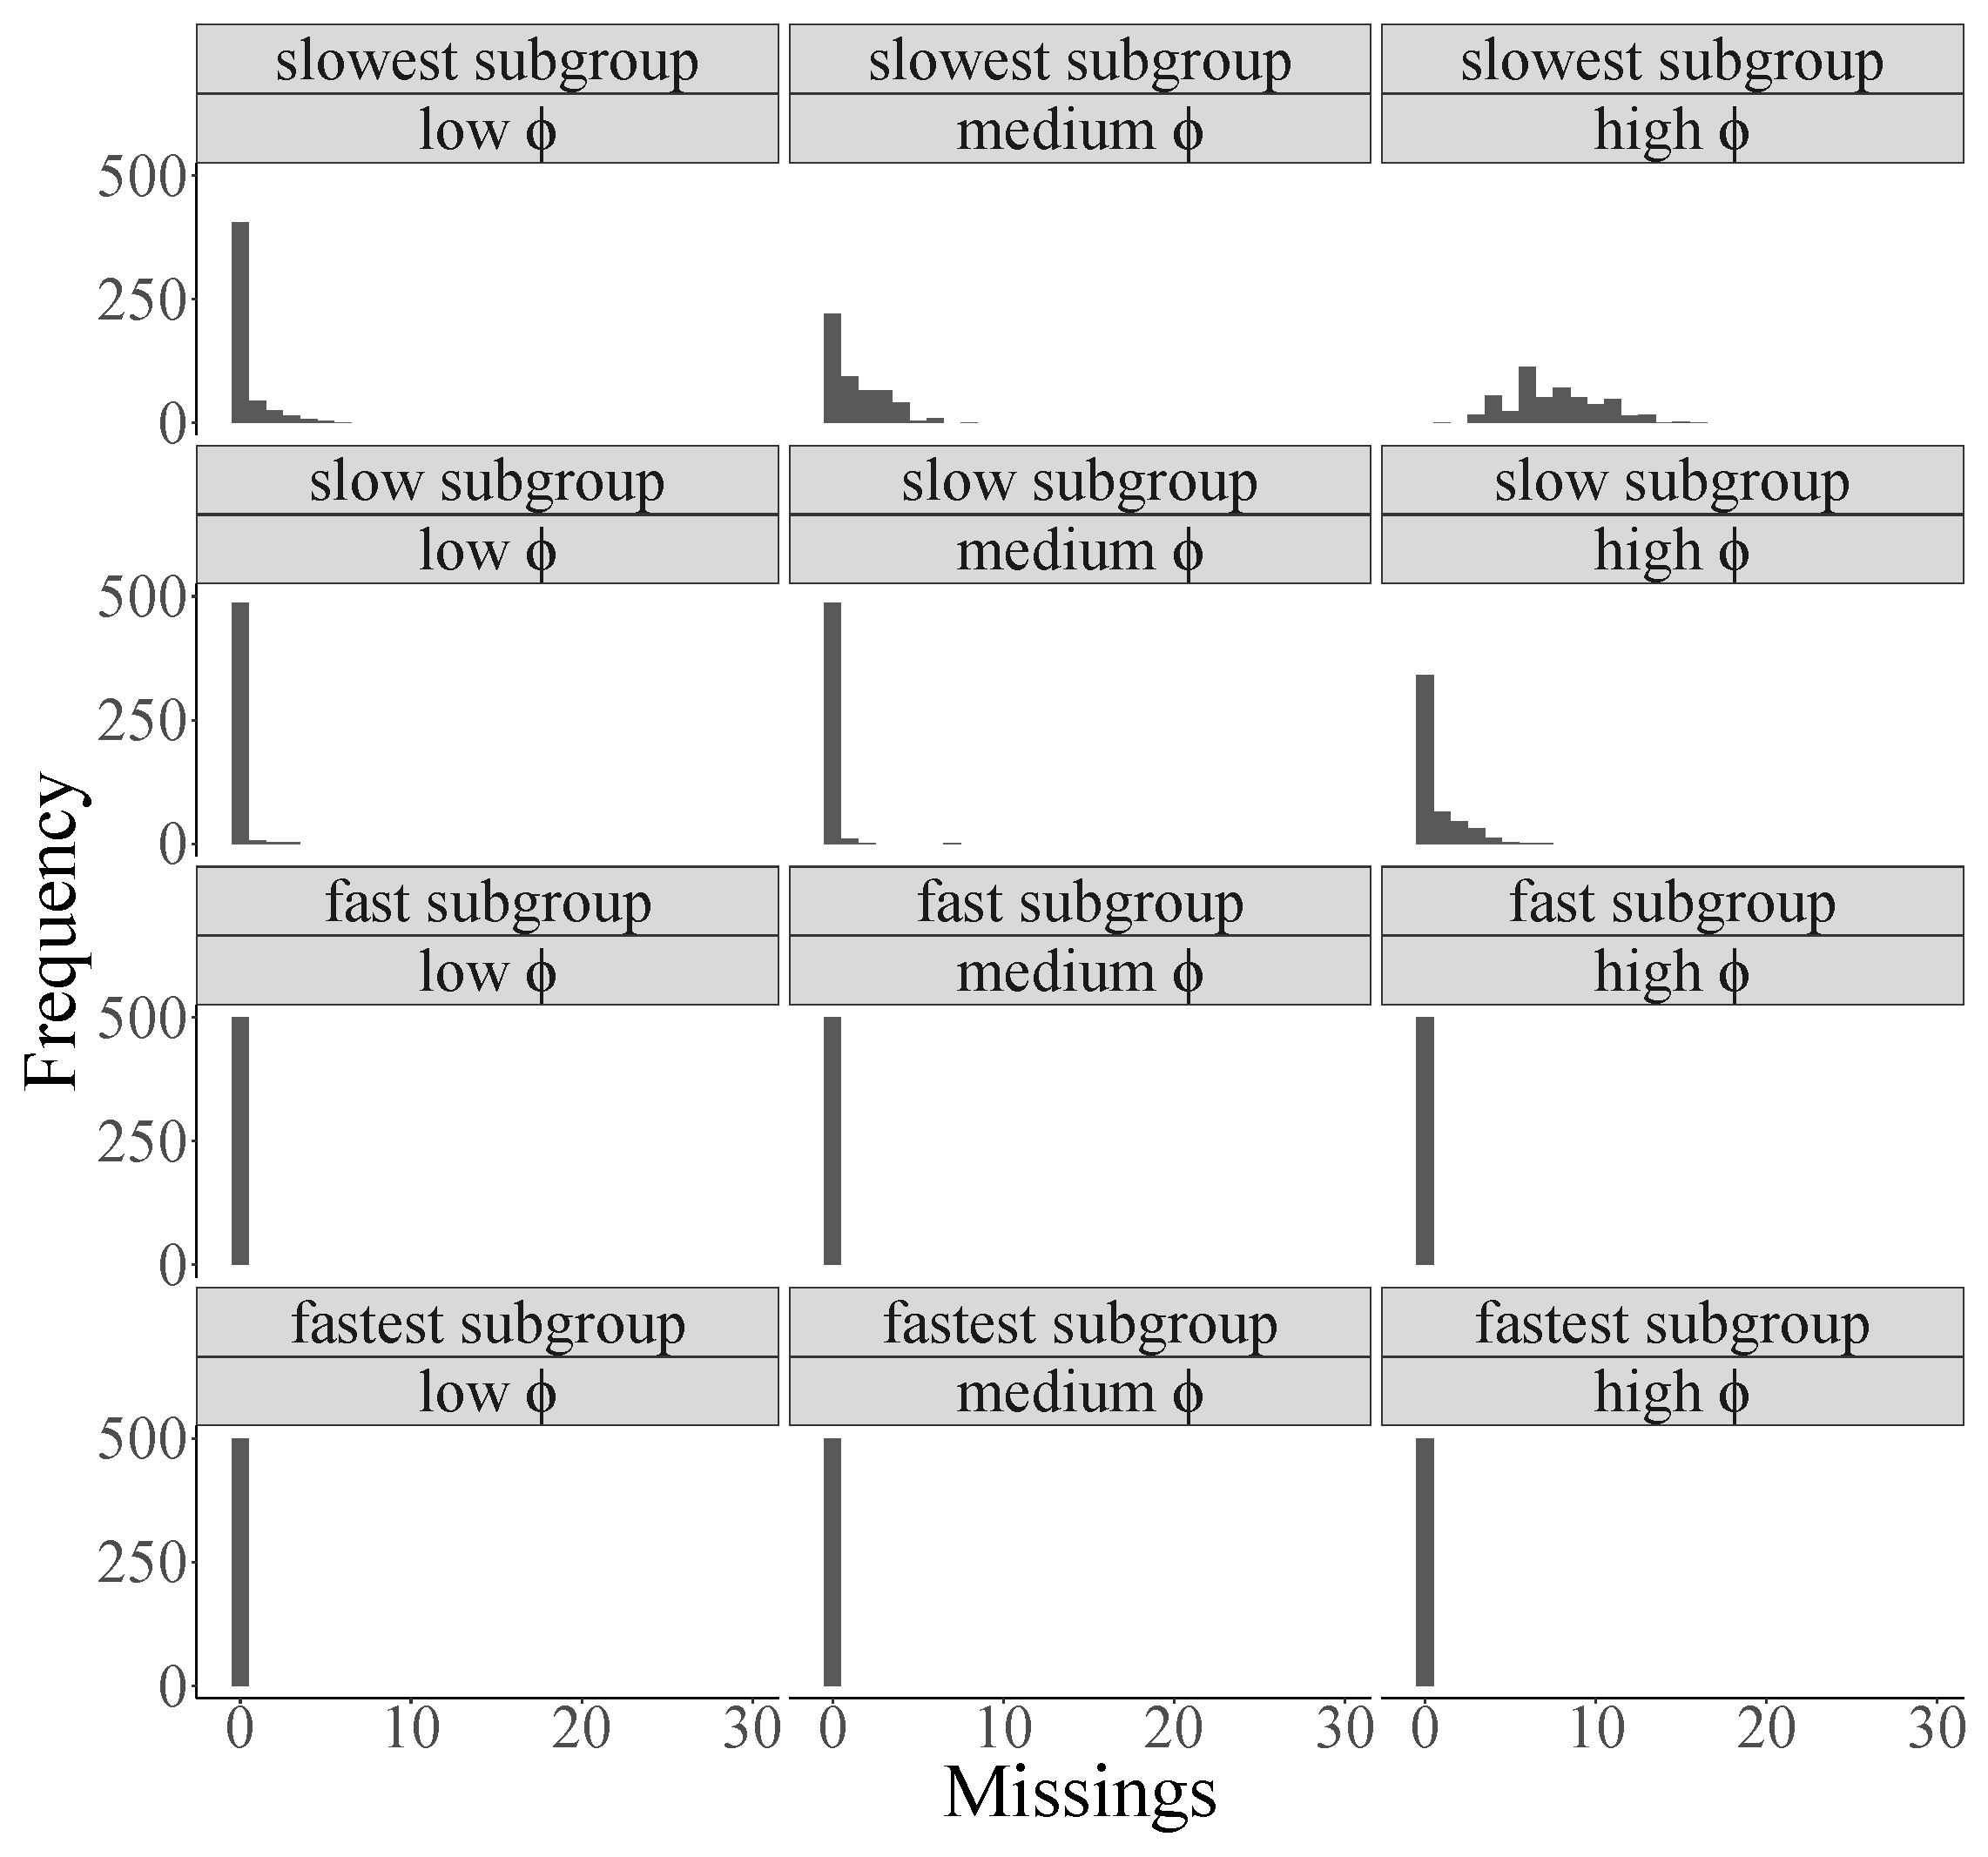
\includegraphics[height = 0.4\textheight]{miss_subGroup.eps}
	\end{center}
		\caption{Number of not reached items for the low, medium and high speed sensitivity test form, across the four subgroups. Results shown for a randomly selected single replication.}	
		\label{fig:miss}
\end{figure}


\section{Standard Deviations for Simulation Results Across Replications}
% latex table generated in R 3.6.2 by xtable 1.8-4 package
% Mon Feb 03 14:11:22 2020
%\begin{sidewaystable}
\begin{table}
\centering
%\rotatebox{90}{ 
%\begin{varwidth}{0.8\textheight}
\caption{Standard Deviations for Test Statistics per Test Form and per Speed Group, Across All Replications.}
\begin{tabular}{llrrrrrrr}
  \hline
Test Form & $\zeta_{i}$ & $M(RT)$ & $SD(RT)$ & $M(mis)$ & $SD(mis)$ & $cor(\theta, \theta)$ & RMSE & $M(\theta_{diff})$ \\ 
  \hline
low $\phi$ & slowest & 42.06 & 31.42 & 0.01 & 0.01 & 0.02 & 0.05 & 0.03 \\ 
  low $\phi$ & slow & 33.39 & 24.36 & 0.00 & 0.01 & 0.01 & 0.05 & 0.02 \\ 
  low $\phi$ & fast & 21.51 & 17.30 & 0.00 & 0.00 & 0.02 & 0.06 & 0.02 \\ 
  low $\phi$ & fastest & 18.04 & 14.39 & 0.00 & 0.00 & 0.02 & 0.06 & 0.02 \\ 
  medium $\phi$ & slowest & 46.88 & 33.10 & 0.02 & 0.02 & 0.02 & 0.07 & 0.05 \\ 
  medium $\phi$ & slow & 33.97 & 25.37 & 0.00 & 0.01 & 0.02 & 0.06 & 0.02 \\ 
  medium $\phi$ & fast & 19.86 & 16.64 & 0.00 & 0.00 & 0.01 & 0.05 & 0.02 \\ 
  medium $\phi$ & fastest & 16.25 & 13.48 & 0.00 & 0.00 & 0.02 & 0.06 & 0.02 \\ 
  high $\phi$ & slowest & 63.29 & 47.33 & 0.04 & 0.02 & 0.04 & 0.15 & 0.14 \\ 
  high $\phi$ & slow & 41.06 & 29.78 & 0.01 & 0.01 & 0.02 & 0.06 & 0.03 \\ 
  high $\phi$ & fast & 17.54 & 13.72 & 0.00 & 0.00 & 0.01 & 0.05 & 0.02 \\ 
  high $\phi$ & fastest & 12.45 & 9.82 & 0.00 & 0.00 & 0.02 & 0.06 & 0.02 \\ 
   \hline
\end{tabular}
%\end{varwidth}}
\begin{tablenotes}
\vspace{0.1cm}
\small
    \textit{Note:} Standard deviations across replications are depicted for mean cumulative response times M($RT$) and the corresponding standard deviation SD($RT$), mean proportion of missings M(mis), the corresponding standard deviation SD(mis), correlation between true and estimated ability $cor(\theta, \theta)$, root mean square error (RMSE) and average difference between true and estimated ability $M(\Delta_{\theta})$. 
\end{tablenotes}
\label{tab:descr}

\end{table}
%\end{sidewaystable}


\begin{flushleft}
\bibliography{../references}
\end{flushleft}


\end{document}